% !TEX root=frame_thesis.tex

\chapter{Introduction}\label{chapter:Introduction}

%First resource are trees, which were cut and used for food production (sweet sap is emerging from cut stems \citet{Mieth2015}), the production of manufactured goods like ropes or tools as well as canoes for fishing, firewood for cooking and cremation and, not to forget, the construction and transport of the Moai (e.g.\ \citet{Diamond2011}). Due to the slow regrowth of the palm tree (e.g. \citet{Brander1998}) this resource is close to non-renewable. Furthermore, the Polynesian rat, introduced by the first settlers at least stopped regrowth of the tree

%Easter Island's suitability for agriculture has been subject to excessive debate not least due to the first very contrary observations made by Roggeveen in 1722 as an `outstandingly fruitful' and by Cook in 1774 as an extremely poor and often sterile island \citep{Bahn2017}. %page 112   % who perceived the island's agricultural potential completely contrary \citep{Cauwe2011}.
%Nevertheless, from archaeological studies we know that the Easter Island people cultivated sweet potato, taro, yam, banans, sugar cane and other crops.
%Since sweet potato appears to be the dominant staple crop \citep{Louwagie2006}, I focus on this single crop here.

%Despite the progress so far, hypothesis  have produced very different results with strong implications on the reconstructed history of the Rapa Nui.

%\section{The Dispute about Pre-historic Easter Island}
%\subsection{Different Theories on the Population Dynamics}
%\begin{itemize}
%	\item Easter Island's Pre-history is a fiercely debated topic
%	\item Different theories exist on the population dynamics \citet{Hunt2007} and \citet{Diamond2011}/\citet{Bahn2017}.
%	\item The differences occur because archaeological data is connected to large uncertainties (e.g.\ tree patterns \citet{Rull2020})
%\end{itemize}
%Malthus
\paragraph{Population Growth and the Malthusian Theory}
Human activity in the recent century has left a pronounced mark on the natural environment such that the term `Anthropocene' is now widely accepted for the current geological epoch.
With exponentially rising concentration of greenhouse gases, plastic pollution, or biodiversity loss (among many other indicators) in a period often denoted as the `Great Acceleration', the human population is becoming a key factor in the environmental dynamics.
One of the most striking and foundational developments in this context is the growth of the global population from less than $2$ to currently $7.8$ billion within a century. 
Given the limited resources of our planet, this development raises concerns about to the carrying capacity of the planet. %potential population overshoot and corresponding fatal consequences for the human society.
One of the first theories proposing an overshooting population was developed by Thomas Malthus.
In \citet{Malthus1798}, he draws a grim picture of a potential anthropogenic trajectory: As the population size grows exponentially, resources such as fertile land exhaust,
leading to increased prices, conflict and the general potential of a collapse of the human society.
Later and with a main focus on environmental degradation, the Club of Rome followed this rationale in their report on `The Limits of Growth' \citep{clubofrome1972}.
Of course, so far no global overshoot has occurred throughout history, as technological advances such as Nitrogen fertilisation have greatly enhanced the planet's population carrying capacity.
Furthermore, it is now more commonly assumed that a global population follows a logistic rather than an exponential growth. 
However, as resources (and eventually also replacements for resources) are limited and conservative projections of a logistic population and resource requirement dynamics can not be safely relied upon, it is only sensible to study the implications for our human society in a scenario of population overshoot, especially with climate change posing a real and imminent threat to the overall livability on the planet \citep{Reuveny2012}.

%If only to be prudent, we must consider whether Malthus basically foresaw a real problem and miscalculated only its geographical scope and timing.


%Instead of trying to predict the dynamics of a global-scale population overshoot in our complex socio-economic system, 
\paragraph{Examples of Overpopulation and Resource Exploitation in Ancient Civilisations}
The disappearance of smaller, ancient civilisations, such as the Maya in Meso-America, the Anasazi in the South West of the United States, or the Norse in Greenland, often in connection to environmental degradation provide interesting case studies.
%\citet{Diamond2011} argues that ancient civilisations  the Maya, the Anasazi, the Norse in Greenland,...
In particular, the fate of the Easter Island civilisation, the `Rapa Nui', has captured scientific and public interest alike for centuries.
One reason is the total isolation of the remote, Pacific island over several centuries, providing an ideal, closed laboratory case of a socio-ecological system.
Another is the substantial environmental change detected on the island following human settlement.  
Within a relatively short period of time, the initial dense palm tree forest turned into barren land deprived of any large vegetation as observed by the first European voyages to the island in the 18th century.
Finally and most importantly, the platforms (`Ahu') and hundreds of infamous statues (`Moai') carved, transported to and erected in various places on the island indicate a large population with rich culture, advanced technological know-how, well established political institutions and a working trading economic system \citep{Cauwe2011}.
This impression is in stark contrast to the observed deforested island, with a relatively small and potentially even rivalrous civilisation reported especially in later visits to the island after $1770\, {\rm A.D.}$.
Resolving this mystery behind the Rapa Nui before European contact has arguably become one of the most interesting anthropological questions.

%Finally the erection of platforms and hundreds of the infamous statues in various places on the island despite the apparent lack of large scale vegetation indicating a rich culture with extensive technological advances, well established 
%and at some point decimated population has posed an unsolved mystery ever since the first European witness reports.
\paragraph{Facts about Easter Island History}
Numerous studies in the fields of archaeology and anthropology have tried to reconstruct the history of the island and its people before European contact.
However, data is often sparse and can be interpreted in various ways \citep{Merico2017}.
E.g.\ many Moai have been toppled in the 18th century which was interpreted as a sign of violence \citep{Bahn2017} or a religious/cultural burial process \citep{Cauwe2011}.
Often theories on the population dynamics are based on pollen records and charcoal data from sediments in the three crater lakes.
However, there are substantial uncertainties in the dating of such data due to the process of sedimentation including geological gaps (\citet{Hunt2007} and \citet{Bahn2017}) and drought periods, in the extrapolation to an island-wide data record \citep{Rull2020} and, most importantly, in the interpretation of these proxies for human activity and, thus, population dynamics on Easter Island (e.g.\  \citep{Cole2008}).
While many aspects of Easter Island history are debated, there are a few typically commonly accepted facts.
The relevant ones for this thesis include:
\begin{itemize}
	\item Before human settlement, the island was forested (\citet{Mieth2015}, \citet{Rull2010}).
	\item Polynesian rats, which were introduced to the island by the first settlers as a protein source, quickly reproduced and effectively hindered the regeneration of palm forests by gnawing on the seeds (\citet{Hunt2007} and \citet{Bahn2017})
	\item Starting from around $1200\,{\rm A.D.}$, there is evidence for intensified deforestation in some places on the island \citep{Rull2020} but with unknown contribution of different drivers (rats, climate or humans).
	\item The Rapa Nui farmed land and cultivated sweet potato, taro, yam and many other crops. They used advanced methods, like lithic mulching, to increase the harvest yields (e.g. \citep{Louwagie2006}). However, the suitability of the soil and climatic conditions for farming remains an open question \citep{Bahn2017}.
	\item The Moai were carved from the 13th to 17th century, followed by a societal change in the 17th or 18th century \citep{Cauwe2011}.
	\item European Voyages arrived in $1722\, {\rm A.D.}$ and more frequently after $1770\, {\rm A.D.}$. They found a (nearly) treeless island and vaguely estimated the population size to be `thousands' in $1722\, {\rm A.D.}$, between $1000$ and $3000$ in the late 18th century and only $111$ in $1872\, {\rm A.D.}$ following devastating slave trade and a smallpox epidemic brought by Europeans \citep{Bahn2017}.
\end{itemize}

\paragraph{Main Uncertainties and Different Narratives of Easter Island History}
The uncertainties in the dynamics of deforestation and population size have lead to two major, contrasting narratives about the natural and anthropogenic contribuitons to deforestation, the correlated population dynamics and, therefore, the overall sustainability of the Easter Island civilisation.
%In order to understand the succession of this diminishing culture, it is interesting to study the succession of events that lead to the extinction to the extinction of a highly 
%but also advanced and labour intensive methods used for cultivating plants on the island by the prehistoric society.
%When the first European voyages discovered the Pacific island in the 18th century, they found a society of a few thousand individuals 
%While we now know that the island must have been densely forested, at the time of discovery the island was nearly deprived of large vegetation.
%Nevertheless, several hundred platforms (`Ahu') and statues (`Moai') were carved, transported and erected in various places on the island.
%Advanced and labour intensive methods for cultivating plants.
%Since then, numerous studies in the fields of archaeology and anthropology have tried to reconstruct the history of the island and its people.
%Two main narratives Easter Island emerged:
On one hand a `genocidal' view \citep{Hunt2007}, on the other hand an `ecocidal' view (\citet{Diamond2011} and \citet{Bahn2017}).
According to the genocidal view, the first settlers arrived around $1200\,{\rm A.D.}$, the population size quickly grew to a plateau of $4,000$ individuals and remained at this level for several centuries. Deforestation is attributed to both human activity but crucially fostered by the fast expansion of the Polynesian rats. 
However, the human society remained mostly resilient to this environmental degradation only to eventually be diminished by the introduction of European diseases and slave trade. 
According to the ecocidal view, the arrival of the first settlers occurred before $1000\, {\rm A.D.}$. 
The population then grew steadily and deforested and burnt trees to clear land for agriculture. This development intensified around $1200\, {\rm A.D.}$. 
Population size peaked some time after $1500\, {\rm A.D.}$ at levels estimated between $6,000$ to $8,000$ or $10,000$ to $20,000$ \citep{Bahn2017}, followed by a steep decline or even `collapse' \citep{Diamond2011} before European contact.
The narrative concludes that the Easter Island population overexploited the natural resources and, consequently, got locked in the Malthusian catastrophe of resource shortage, cultural disruption, conflict and consequent population decrease.
%page 218
Next to these two major themes, various other theories have been put forward.
\citet{Brandt2015} suggest a quick population growth followed by a slow-demise in their modelling study.
A model developed by \citet{Cole2008} suggests multiple periods of growth and collapse throughout history. 
Furthermore, \citet{Rull2016} reviews evidence for climatological impact rather than anthropogenic drivers of the deforestation, arguing for a more holistic perspective on Easter Island.
The dynamics of population size and deforestation and its causes remain a fiercly debated topic as the different narratives strongly correlate with our impression of the Rapa Nui in the face of an environmental crisis. 


%according to which the society was resilient in the face of a rat-induced deforestation but was eventually diminished due to the introduction of European diseases, and an ecocidal view, according to which humans  overexploited their dominant resources and found themselves faced with a declining population size \citep{Bahn2017} or even a collapse \citet{Diamond2011} with various socio-political consequences.
%Other theories include a slow-demise 
%Climate 

\paragraph{Mathematical Modelling of Socio-Economic Systems of Ancient Societies}
Easter Island history is studied in various disciplines, from archaeologists to anthropologists. 
A major contribution, however, has also been made by the field of socio-economic modelling of ancient societies.
Mathematical modelling, typically with macroscopic system models, has helped to explain, rule out or propose possible or realistic scenarios of natural and anthropogenic dynamics on Eater Island given a certain set of assumptions.
I describe these models of Eater Island in more detail in Chapter \ref{chapter:Theory}, and describe how they share the same insufficiencies.
In this thesis, therefore, I take a different approach for a mathematical, socio-economic model of Easter Island, an Agent-Based Model, to understand the implications and constraints to the spatial and temporal patterns of the civilisation and the environment in the face of microscopic, individual behaviour and uncertainty.

\paragraph{Outline}
In Chapter \ref{chapter:Theory}, I describe both types of mathematical models, the various existing macroscopic system models and the new approach of Agent-Based Modelling pursued in this thesis.
%I continue by pointing out shortcomings in the approaches used so far and explain the need for an Agent Based Model.
In Chapter \ref{chapter:Methods}, I develop such an Agent-Based Model from scratch by defining a spatially explicit environment, human agents with specific features and their various actions and interactions. 
I also justify the choices and assumptions made in this model with the existing literature (and plausiblity, where necessary).
In Chapter \ref{chapter:Results}, I then present some results obtained with this model and discuss the implications for the spatio-temporal history of Easter Island given variations of modules and parameters in the model.

\chapter{Mathematical Theory}\label{chapter:Theory}
\FloatBarrier
\section{Macroscopic, Differential Equation Based Approaches for Easter Island}
%\begin{itemize}
%	\item Mathematical modelling has helped to explain possible scenarios of the dynamics and give interpretations of the historical developments.
%	\item So far, all mathematical models focus on differential equation based approaches for the aggregate population of Easter Island.
%	\item \citet{Brander1998}
%	\item Variations of \citet{Brander1998}: Summarise the reviews in \citet{Reuveny2012}, \citet{Merico2017}.
%	\item Social institution Extension of \citet{Brander1998}: \citet{Good2006}.
%	\item Spatial Diffusion and Rats extension of \citet{Brander1998}: \citet{Basener2008}.
%	\item The problem of these models is that with little variation in the parameters, any population dynamics can be achieved \citep{Brandt2015}.
%\end{itemize}

\paragraph{The Basic Ordinary Differential Equation Model}
A theory about population dynamics and deforestation on Easter Island is often supported by a mathematical, human-resource interaction model.
%By making assumptions about these interaction sometimes based on archaeological data, these models can produce realistic population dynamics and thereby explain or rule out certain scenarios under the used set of assumptions. 
So far, all of those models are based on aggregate predator-prey type of interaction between humans and resources provided by the environment (so called Lotka-Voltera model).
The dynamics of these macroscopic variables is then described by often non-linear, coupled ordinary differential equations (ODE).
The first and most famous model was developed by \citet{Brander1998}. 
The authors simulate the dynamics of two variables, an exponentially growing human population size $L$ (the predator) and a logistically growing open-access resource with stock $S$ (the prey).
This resource can be interpreted as the forest/soil complex, which is slowly renewable in this model. 
Of course, the Rapa Nui did not live off trees.
However, the palm tree forest provided valuable derivate products or ecosystem services (e.g.\ as habitat for birds, firewood, technical wood for tools or the transport of the Moai statues, or even as a supplement for freshwater \citep{Bahn2017}) and is, thus, often considered as the primary resource in Easter Island models.
Consumption of the resource enables population growth and thus, the human population harvests $H(L,S)$ from the resource, and thereby depletes its stock.
The set of ODEs is
\begin{eqnarray}\label{eq:Brander}
\frac{dL}{dt} = L \cdot (b-d) + \phi \cdot H(L,S) \\
\frac{dS}{dt} = G(S)\cdot S - H(L,S) \ ,
\end{eqnarray}
where $b$ and $d$ are the constant birth and death rates, $\phi$ denotes the increase of fertility with resource consumption and $G(S)$ is the logistic growth rate of the resource.
This model applied to Easter Island reproduced a `boom and bust' cycle (Figure \ref{fig:brander1998eibasecase}), which as they argue is an example of the `Malthusian forces [leading] to a depletion of the resource base and social conflict' and thereby supports the ecocidal view of Easter Island history.
\begin{figure}
	\centering
	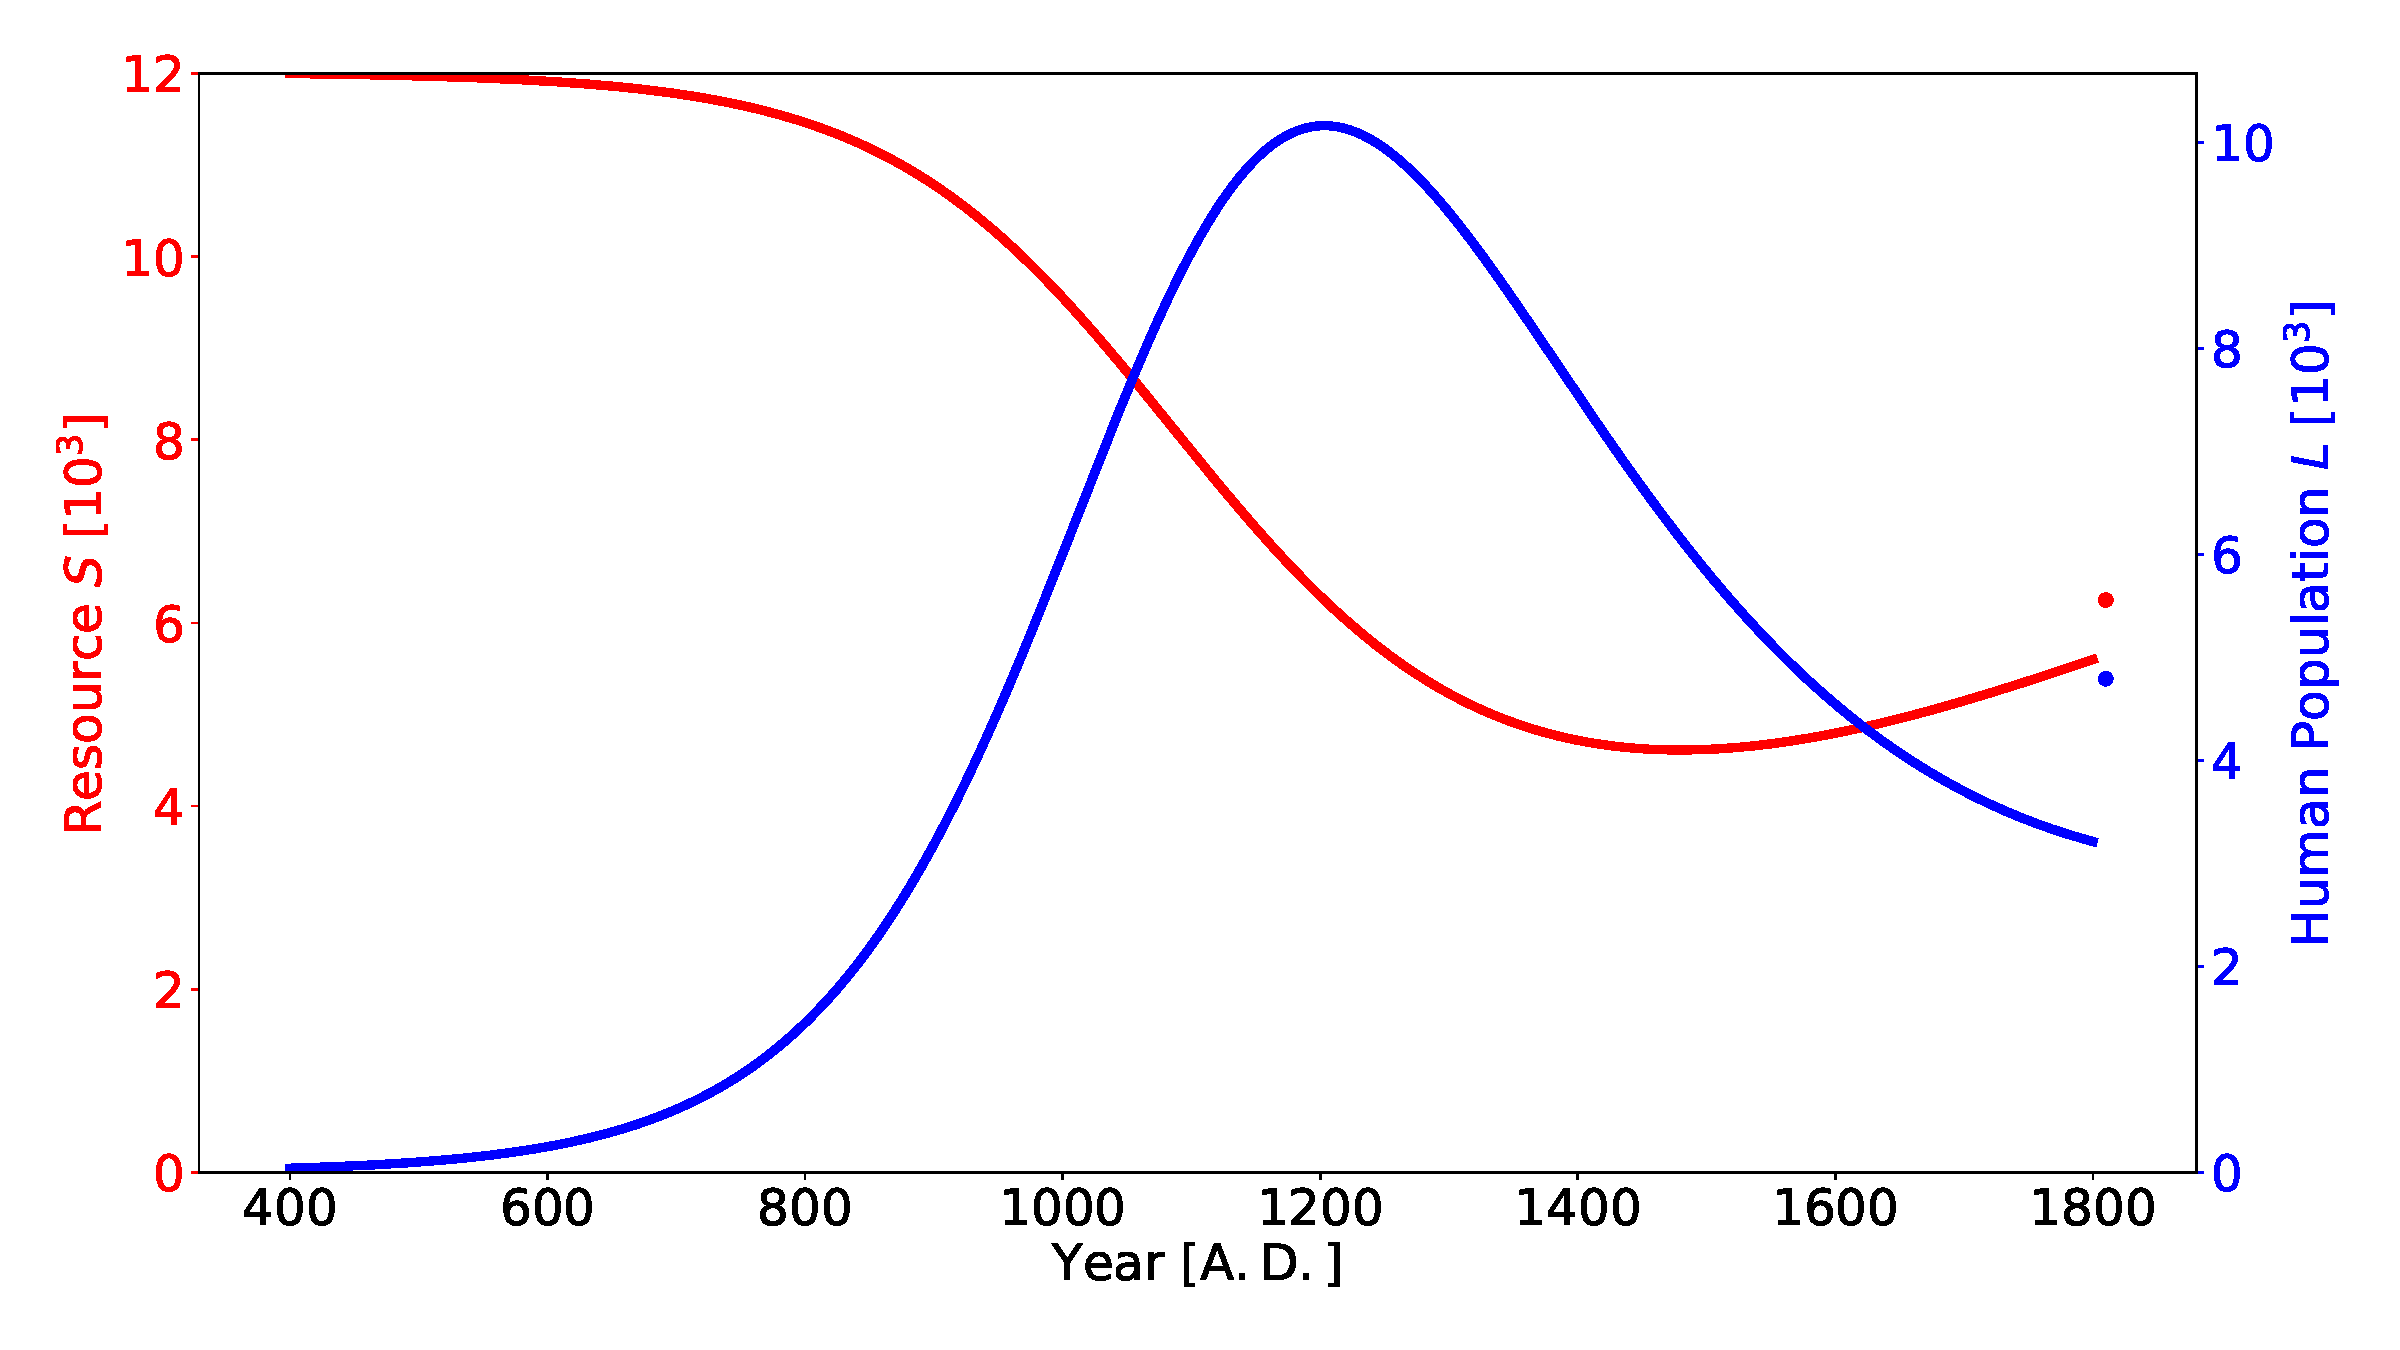
\includegraphics[width=1 \textwidth]{images/Brander1998_EIBaseCase}
	\caption{Replication of the model in \citet{Brander1998} with parameter setting as in the `Easter Island Base Case' in Figure 3 of the publication. The dots on the right represent the equilibrium values.}
	\label{fig:brander1998eibasecase}
\end{figure}

\paragraph{Extensions of the Basic Model}
In the last two decades several extensions and adjustments have been added to the first mathematical model by \citet{Brander1998}.
\citet{Reuveny2012} provides an extensive overview of these models.
\citet{Merico2017} additionally summarises gaps and advances within this field of research. 
Here, I point out those models relevant to the motivation for this thesis.
\citet{dAlessandro2007} separates the resource dependency from one single stock to two, an inexhaustible and a renewable resource (that irreversibly exhausts if below a certain threshold).
The author finds multiple stable states due to this disaggregation of the ecological variable. 
A model by \citet{Good2006} introduces foresight and resource management institutions (either a system of property rights or a social planner) to the simple predator-prey harvest in \citet{Brander1998}.
Here, the society's harvest rate is determined by maximising a utility function over a certain time horizon with reasonable discounting (e.g.\ by a social planner which could be an emergent political hierarchy).
However, the authors find that even with optimal institutions in place, collapse of the Rapa Nui population size is inevitable.
\citet{Basener2008} added another variable to the model next to tree number and human population size, which accounts for the rat population and their devastating impact on tree regrowth as previously found by \citet{Hunt2007}. 
This model was then further extended by a spatial component \citep{Basener2011}. 
A number of homogeneous, one-dimensional cells was defined and diffusion of rats and humans allowed between adjacent cells. 
The authors find that simply changing the mobility of rats can qualitatively alter the dynamics of the human population size.
While this representation is extremely simplified and the diffusion process is unintuitive for human settlement pattern of a small island, this is the only model on Easter Island including a physical space to my knowledge.
Finally, in a recent analysis, \citet{Brandt2015} extended the model of trees, rats and humans by \citet{Basener2008} with a disease spreading model.
They found that the model can obtain any of the proposed narratives (ecocide, genocide or the slow-demise) through variation of only a few parameters in a reasonable range.
All of these various models build on the basic assumptions by the basic processes described in the macroscopic ODE model by \citet{Brander1998}.


\paragraph{Shortcomings of Macroscopic ODE Models}
Despite the extensive body of research presented by the numerous macroscopic system models on Easter Island, the dispute between different narratives could not be put aside.
The ODE based models, the main tool for Easter Island modelling, typically either showed the same (inherent) boom and bust cycle or showed shortcomings in that different choices of parametrisation within the uncertainties of the sparse archaeological data consistently lead to contrasting results and narratives.
%ODE-type modelling can only have limited significance.
Many shortcomings of these models are inherent problems of macroscopic system modelling, e.g.\ the missing spatial constraints, heterogeneity, co-evolving behaviour and emergent phenomena.
A microscopic, agent-based model therefore builds a useful alternative to these macroscopic ODE model approaches in addressing many of the problems as described in the next Section.
%E.g.\ the model by \citet{Brander1998} assumes open access to the resources which defers intuition since the location of an individual restricts the availability of resources. 
%Other models \citep{Good2006} might include a more complex economic which incorporates restrictions on resource harvest but implemented via a social planner.
%Thus, such dynamics are not co-evolving or emergent but externally established 

%While models like \citet{Good2006} have restrictions on the amount of resources, it require a social planner and it is not so much an emergent restriction of the population dyanmics but rather a institution.

\FloatBarrier
\section{Agent-Based Modelling (ABM) of Human-Resource Interactions -- Overview, Motivation and Previous Approaches}
%\begin{itemize}
%\item What is Agent Based Modelling
%\item The basic structure of an ABM in human resource interactions: Agents in environment, Update all agents asynchronously, update environment. Within each update agents change their local environment and their behaviour/properties are in turn influenced by the local environment. 
%\item It breaks with ODE-type of modeling because it enables: 
%\begin{itemize}
%	\item spatially explicit modelling,
%	\item  emergent global behaviour from local rules, 
%	\item computational irreducibility of agent behaviour in terms of crisis. 
%	\item Non-ergodic relation between agents and their environment.
%	\item Stochasticity is natural in the decision making process, due to an agent's imperfect knowledge of the global sitution
%\end{itemize}
%\item ABM in ancient historical population dynamics: Maya \citep{Heckbert2013} and Anasazi \citep{Axtell2002}
%\item Why ABM could help in Easter Island modelling: \citet{Merico2017}.
%\item Structure of this thesis.
%\end{itemize}

\paragraph{Overview of ABM}
Agent-Based Modelling (ABM) is now a common tools at the centre between cognitive psychology, game theory and complexity science \citep{Bousquet2004} with roots in the field of Artificial Intelligence.
In Agent-Based Models (ABMs) a system is grown bottom-up from its constituent units.
Hence, the perspective of an ABM therefore focuses on the microscopic rather than macroscopic system.
An ABM (as used in this thesis) simulates a number of discrete agents (e.g.\ humans), often situated in an environment, with specific traits.
Agents (and the environment) are updated asynchronously at certain timesteps over the simulated period.
In each update, a single agent interacts with the environment and other agents according to a set of individual rules.
These rules are usually heterogeneous, non-linear (e.g.\ discontinuous or discrete), stochastic, time-dependent and adaptive and might be memory- and path-dependent \citep{Bonabeau2002}.
In the case of a spatial model, rules and behaviour additionally depend on the explicit location of an agent in the environment.
Usually, agents make individual decisions, based on perceptions of their local surroundings and their internal state, and thereafter act independently and autonomously.
With this microscopic setup, overall macroscopic dynamics of the system are obtained.
Aggregate system variables can then be interpreted both as outcomes of and as contexts for the agents' decisions and actions \citep{Kohler2000}.
The analysis of system variables and, therefore, the ABM is not straight-forward, however, especially if the model does not serve a general purpose and can be greatly simplified.
In fact, validation of an ABM is classically done by simply running simulations (enabled by the rise of computational power in the recent decades) and comparing them with observations \citep{Bousquet2004}.

%The field of Agent Based Modelling originally comes from Artificial Intelligence study. 
% WHERE FROM 
% INFORMATICS, EXAMPLES, ...


%These are updated asynchronously in certain timesteps over the simulation period. 
%In each update, a single agent interacts with the environment and other agents and adapts its own features.
%Usually, agents act independently and based on individual decision making by evaluating their state at the current time.
%Aggregate variables of all agents are then a combination of context as well as outcome \citep{Kohler2000}.



\paragraph{Advantages with respect to ODE Models}
In many complex systems, ABMs are advantageous over macroscopic system models by accounting for the following system properties \citep{Bookstaber2019}:
\begin{itemize}
	\item Emergent phenomena from local, heterogeneous behaviour of the agents,
	\item Computational irreducibility of agent behaviour (e.g.\ in the decision making in times of crisis),
	\item Non-ergodicity of relations between agents and their environment (i.e.\ conditions and rules of behaviour co-evolve with the agent and environment \citep{Kohler2000}),
	\item Stochasticity in the actions and decision making processes, due to imperfect knowledge or uncertainty of the agents. 
\end{itemize}
Additionally, ABMs allow for a very natural and flexible implementation\footnote{Compare for example with the unintuitive diffusion process in the ODE model by \citet{Basener2011}.} of an explicit space dependency of rules and a spatially heterogeneous environment
%In ODE models, space dependency is typically implemented via non-intuitive, complex diffusion processes (compare to the model by \citet{Basener2011}).
%In such systems, ABMs are often the most natural and flexible way of describing a system.
%An ABM is especially relevant if a system exhibits emergent phenomena, i.e.\ individual behaviour according to rules cummulates in complex macroscopic patterns.
In particular, if a system exhibits emergent phenomena, crucial information is lost when the heterogeneity of agents is reduced to one representative agent by averaging, as done in macroscopic ODE models \citep{Bonabeau2002}.
Instead, an ABM generates emergence from bottom-up by accounting for non-linear feedbacks due to heterogeneous agents and stochasticity e.g.\ connected to uncertainty in the decision making process.

%Furthermore stochastic, discrete processes as in an ABM lead to complex responses of the model outcome, that can not be simply 
% while an ABM gives rise to non-linear feedbacks of fluctuations e.g.\ in the case of uncertainty.
%In such cases, simple averaging and expressing processes by a representative behaviour, as applied in macroscopic system modelling, does not capture emergent phenomena.
%However, an ABM gives rise to non-linear feedbacks from heterogeneous, fluctuating agents e.g.\ in the face of uncertainty and imperfect knowledge in decision making.


\paragraph{Application in Socio-Ecological Systems}
ABMs have traditionally been applied to problems connected to flows, markets, organisations, or diffusion \citep{Bonabeau2002}.
Typical applications include e.g.\ traffic jams, ant colonies or swarm behaviour of fish and bird flocks.
However, ABMs are also a common approach for socio-ecological systems \citep{Muller-Hansen2017}.
Such a system comprises complex, co-evolution of the heterogeneous humans and environment, which interact with each other in non-linear, adaptive interactions on multiple time and spatial scales, making it a suitable for the application of ABMs \citep{Bousquet2004}.

%The population dynamics of ancient societies 
%, as agents in such a system usually also act heterogeneously and dependent on local space.
%Here, social structure such as the emergence of political organisations in the agent-agent interactions are at the heart of Agent-Based models.
%As agents in ecological systems usually act heterogeneously and strongly dependent on their local environment or neighbourhood, the usage of ABM with an explicit space dependency is suitable \citet{Bousquet2004}.
% motivates the use of ABM in ecological modeling with the local response 

%According to \citet{Bousquet} ABMs in the ecosystem context can be applied to either create scenarios showing `what might be rather than what is' to understand a system or to produce reality-like scenarios in order to test `what if' questions.

%The disadvantage of ABM is that there's no mathematical proof.Bousquet2004.

\paragraph{Appication for Ancient Civilisations}
Agent-Based Modelling has also been applied to study the history of two ancient civilisations.
Firstly, \citet{Axtell2002} (and \citet{Janssen2009}), use an ABM to reproduce the spatio-temporal history of the Anasazi society in a valley in Arizona, US, and its disappearance around $1300\, {\rm A.D.}$. 
Agents in the model represent households with various heterogeneous attributes that interact with the environment via farming. 
The environment is determined from an extensive data record of harvest yield potential in the valley over time and the Agent-Environment interaction bases on this yield and a set of anthropologically plausible rules.
Agents choose a location for a farm depending on the maximum potential yield in a certain distance to water and for the nearest possible settlement with access to water. The harvest success determines the fertility and thus the dynamics of agent numbers and overall population in the valley.
Secondly, \citet{Heckbert2013} develops an ABM for the Maya civilisation resulting in a `somewhat analogous' reproduction of the spatial pattern and timeline.
The agents in this model generate a certain amount of agricultural yield on cells of a discretised map based on a benefit-cost assessment. 
They are further connected in clustered, adaptive trade networks, from which they benefit.
Both of these approaches by \citet{Axtell2002} and \citet{Heckbert2013} attempt to explain the spatio-temporal history of an ancient civilisation by growing an Agent-Based Model with anthropological rules and a biologically, geographically explicit environment on a discretised map.


\paragraph{Motivation for applying an ABM on Easter Island}
This thesis presents a similar Agent-Based modelling approach for the history of Easter Island.
I have discussed many aspects and advantages of ABM, which apply in socio-ecological systems, and for modelling ancient societies (and Easter Island in particular).
Similar to the valley of the Anasazi, Easter Island is a small, confined space with distinct geographical and biological features with heterogeneous agricultural suitability.
\citet{Merico2017} further argues for the use of an ABM for Easter Island to overcome the shortcomings of ODE models and limits of the available archaeological data.
The main features of the ABM presented here, thus, include a spatially explicit environment, locally confined agent-environment interaction, a simple adaption strategy of agents to environmental degradation and individual, stochastic moving decisions by agents.

